\chapter{2 Samuel 22}

\begin{figure}
  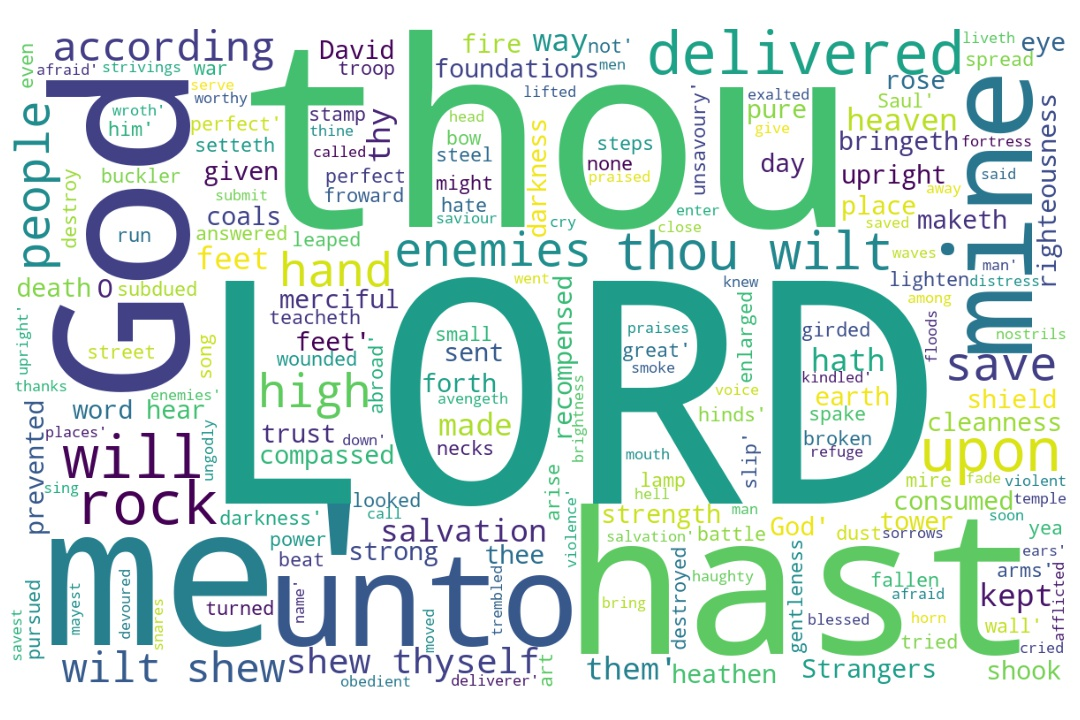
\includegraphics[width=\linewidth]{10OT-2Samuel/2Samuel22-WordCloud.jpg}
  \caption{1 Samuel 22 Word Cloud}
  \label{fig:1 Samuel 22 Word Cloud}
\end{figure}

%%%%%%%%%%%%%%%%%%%%%%%%%%%%%%%%%%%%%%%%%
%%%%%%%%%%%%%%%%%%%%%%%%%%%%%%%%%%%%%%%%%

\marginpar{\scriptsize \centering \fcolorbox{bone}{lime}{\textbf{DAVID"S REFLECTION}}\\ (2 Samuel 22:1--51) 
\begin{compactenum}[I.][8]
    \item David as a  \textbf{Vessel} %\index[scripture]{2Samuel!2Sa 22:01}(2Sa 22:1) 
    \item Two \textbf{Voices}  \index[scripture]{2Samuel!2Sa 22:07}  \index[scripture]{2Samuel!2Sa 22:14} (2Sa 22:7, 14) 
    \item The \textbf{Virtue} (or lack thereof, and the rewards thereof, but the repentance \index[scripture]{2Samuel!2Sa 22:22--26}(2Sa  22:22--26) 
    \item God's Care for \textbf{Victims}  \index[scripture]{2Samuel!2Sa 22:28}(2Sa 22:28) 
    \item The \textbf{Victories}  \index[scripture]{2Samuel!2Sa 22:40}(2Sa 22:40) 
    \item An \textbf{Avenging}  \index[scripture]{2Samuel!2Sa 22:48}(2Sa 22:48) 
    \item Deliverance from the  \textbf{Violent}  \index[scripture]{2Samuel!2Sa 22:49}(2Sa 22:49) 
\end{compactenum} }

\footnote{\textcolor[cmyk]{0.99998,1,0,0}{\hyperlink{TOC}{Return to end of Table of Contents.}}}\footnote{\href{https://audiobible.com/bible/2_samuel_22.html}{\textcolor[cmyk]{0.99998,1,0,0}{2 Samuel 22 Audio}}}\textcolor[cmyk]{0.99998,1,0,0}{And David spake unto the LORD the words of this song in the day \emph{that} the LORD had delivered him out of the hand of all his enemies, and out of the hand of Saul:}
[2] \textcolor[cmyk]{0.99998,1,0,0}{And he said, The LORD \emph{is} my rock, and my fortress, and my deliverer;}
[3] \textcolor[cmyk]{0.99998,1,0,0}{The God of my rock; in him will I trust: \emph{he} \emph{is} my shield, and the horn of my salvation, my high tower, and my refuge, my saviour; \fcolorbox{bone}{bone}{thou}  savest me from violence.}
[4] \textcolor[cmyk]{0.99998,1,0,0}{I will call on the LORD, \emph{who} \emph{is} worthy to be praised: so shall I be saved from mine enemies.}
[5] \textcolor[cmyk]{0.99998,1,0,0}{When the waves of death compassed me, the floods of ungodly men made me afraid;}
[6] \textcolor[cmyk]{0.99998,1,0,0}{The sorrows of hell compassed me about; the snares of death prevented me;}
[7] \textcolor[cmyk]{0.99998,1,0,0}{In my distress I called upon the LORD, and cried to my God: and he did hear \fcolorbox{bone}{lime}{my voice} out of his temple, and my cry \emph{did} \emph{enter} into his ears.}
[8] \textcolor[cmyk]{0.99998,1,0,0}{Then the earth shook and trembled; the foundations of heaven moved and shook, because he was wroth.}
[9] \textcolor[cmyk]{0.99998,1,0,0}{There went up a smoke out of his nostrils, and fire out of his mouth devoured: coals were kindled by it.}
[10] \textcolor[cmyk]{0.99998,1,0,0}{He bowed the heavens also, and came down; and darkness \emph{was} under his feet.}
[11] \textcolor[cmyk]{0.99998,1,0,0}{And he rode upon a cherub, and did fly: and he was seen upon the wings of the wind.}
[12] \textcolor[cmyk]{0.99998,1,0,0}{And he made darkness pavilions round about him, dark waters, \emph{and} thick clouds of the skies.}
[13] \textcolor[cmyk]{0.99998,1,0,0}{Through the brightness before him were coals of fire kindled.}
[14] \textcolor[cmyk]{0.99998,1,0,0}{The LORD thundered from heaven, and the most High uttered \fcolorbox{bone}{lime}{his voice}.}
[15] \textcolor[cmyk]{0.99998,1,0,0}{And he sent out arrows, and scattered them; lightning, and discomfited them.}
[16] \textcolor[cmyk]{0.99998,1,0,0}{And the channels of the sea appeared, the foundations of the world were discovered, at the rebuking of the LORD, at the blast of the breath of his nostrils.}
[17] \textcolor[cmyk]{0.99998,1,0,0}{He sent from above, he took me; he drew me out of many waters;}
[18] \textcolor[cmyk]{0.99998,1,0,0}{He delivered me from my strong enemy, \emph{and} from them that hated me: for they were too strong for me.}
[19] \textcolor[cmyk]{0.99998,1,0,0}{They prevented me in the day of my calamity: but the LORD was my stay.}
[20] \textcolor[cmyk]{0.99998,1,0,0}{He brought me forth also into a large place: he delivered me, because he delighted in me.}
[21] \textcolor[cmyk]{0.99998,1,0,0}{The LORD rewarded me according to my righteousness: according to the cleanness of my hands hath he recompensed me.}
[22] \textcolor[cmyk]{0.99998,1,0,0}{For I have kept the ways of the LORD, and have \fcolorbox{bone}{lime}{not wickedly departed} from my God.}
[23] \textcolor[cmyk]{0.99998,1,0,0}{For all his judgments \emph{were} before me: and \emph{as} \emph{for} his statutes, I did not depart from them.}
[24] \textcolor[cmyk]{0.99998,1,0,0}{I was also upright before him, and have kept myself from mine iniquity.}
[25] \textcolor[cmyk]{0.99998,1,0,0}{Therefore the LORD hath recompensed me according to my righteousness; according to my cleanness in his eye sight.}
[26] \textcolor[cmyk]{0.99998,1,0,0}{With the merciful \fcolorbox{bone}{bone}{thou}  wilt shew thyself merciful, \emph{and} with the upright man \fcolorbox{bone}{bone}{thou}  wilt shew thyself upright.}
[27] \textcolor[cmyk]{0.99998,1,0,0}{With the pure \fcolorbox{bone}{bone}{thou}  wilt shew thyself pure; and with the froward \fcolorbox{bone}{bone}{thou}  wilt shew thyself unsavoury.}
[28] \textcolor[cmyk]{0.99998,1,0,0}{And \fcolorbox{bone}{lime}{the afflicted people} \fcolorbox{bone}{bone}{thou}  wilt save: but thine eyes \emph{are} upon the haughty, \emph{that} \fcolorbox{bone}{bone}{thou}  mayest bring \emph{them} down.}
[29] \textcolor[cmyk]{0.99998,1,0,0}{For \fcolorbox{bone}{bone}{thou}  \emph{art} my lamp, O LORD: and the LORD will lighten my darkness.}
[30] \textcolor[cmyk]{0.99998,1,0,0}{For by thee I have run through a troop: by my God have I leaped over a wall.}
[31] \textcolor[cmyk]{0.99998,1,0,0}{\emph{As} \emph{for} God, his way \emph{is} perfect; the word of the LORD \emph{is} tried: he \emph{is} a buckler to all them that trust in him.}
[32] \textcolor[cmyk]{0.99998,1,0,0}{For who \emph{is} God, save the LORD? and who \emph{is} a rock, save our God?}
[33] \textcolor[cmyk]{0.99998,1,0,0}{God \emph{is} my strength \emph{and} power: and he maketh my way perfect.}
[34] \textcolor[cmyk]{0.99998,1,0,0}{He maketh my feet like hinds' \emph{feet}: and setteth me upon my high places.}
[35] \textcolor[cmyk]{0.99998,1,0,0}{He teacheth my hands to war; so that a bow of steel is broken by mine arms.}
[36] \textcolor[cmyk]{0.99998,1,0,0}{Thou hast also given me the shield of thy salvation: and thy gentleness hath made me great.}
[37] \textcolor[cmyk]{0.99998,1,0,0}{Thou hast enlarged my steps under me; so that my feet did not slip.}
[38] \textcolor[cmyk]{0.99998,1,0,0}{I have pursued mine enemies, and destroyed them; and turned not again until I had consumed them.}
[39] \textcolor[cmyk]{0.99998,1,0,0}{And I have consumed them, and wounded them, that they could not arise: yea, they are fallen under my feet.}
[40] \textcolor[cmyk]{0.99998,1,0,0}{For \fcolorbox{bone}{bone}{thou}  hast girded me with strength to battle: them that rose up against me \fcolorbox{bone}{lime}{hast \fcolorbox{bone}{bone}{thou}  subdued} under me.}
[41] \textcolor[cmyk]{0.99998,1,0,0}{Thou hast also given me the necks of mine enemies, that I might destroy them that hate me.}
[42] \textcolor[cmyk]{0.99998,1,0,0}{They looked, but \emph{there} \emph{was} none to save; \emph{even} unto the LORD, but he answered them not.}
[43] \textcolor[cmyk]{0.99998,1,0,0}{Then did I beat them as small as the dust of the earth, I did stamp them as the mire of the street, \emph{and} did spread them abroad.}
[44] \textcolor[cmyk]{0.99998,1,0,0}{Thou also hast delivered me from the strivings of my people, \fcolorbox{bone}{bone}{thou}  hast kept me \emph{to} \emph{be} head of the heathen: a people \emph{which} I knew not shall serve me.}
[45] \textcolor[cmyk]{0.99998,1,0,0}{Strangers shall submit themselves unto me: as soon as they hear, they shall be obedient unto me.}
[46] \textcolor[cmyk]{0.99998,1,0,0}{Strangers shall fade away, and they shall be afraid out of their close places.}
[47] \textcolor[cmyk]{0.99998,1,0,0}{The LORD liveth; and blessed \emph{be} my rock; and exalted be the God of the rock of my salvation.}
[48] \textcolor[cmyk]{0.99998,1,0,0}{It \emph{is} God that \fcolorbox{bone}{lime}{avengeth} me, and that bringeth down the people under me,}
[49] \textcolor[cmyk]{0.99998,1,0,0}{And that bringeth me forth \fcolorbox{bone}{lime}{from mine enemies}: \fcolorbox{bone}{bone}{thou}  also hast lifted me up on high above them that rose up against me: \fcolorbox{bone}{bone}{thou}  hast delivered me from the violent man.}
[50] \textcolor[cmyk]{0.99998,1,0,0}{Therefore I will give thanks unto thee, O LORD, among the heathen, and I will sing praises unto thy name.}
[51] \textcolor[cmyk]{0.99998,1,0,0}{\emph{He} \emph{is} the tower of salvation for his king: and sheweth mercy to his anointed, unto David, and to his seed for evermore.}